% Author: Izaak Neutelings (October 2020)
\documentclass[border=3pt,tikz]{standalone}
\usepackage{physics}
\usepackage{tikz}
\usetikzlibrary{calc}
\usetikzlibrary{angles,quotes} % for pic
\usetikzlibrary{arrows.meta}
\usetikzlibrary{patterns}
\tikzset{>=latex} % for LaTeX arrow head

\colorlet{xcol}{blue!70!black}
\colorlet{vcol}{green!60!black}
\colorlet{myred}{red!65!black}
\colorlet{mypurple}{blue!60!red!80}
\colorlet{acol}{red!50!blue!80!black!80}
\tikzstyle{rvec}=[->,xcol,very thick,line cap=round]
\tikzstyle{vvec}=[->,vcol,very thick,line cap=round]
\tikzstyle{myarr}=[{Latex[length=3,width=3]}-,xcol]
\tikzstyle{force}=[->,myred,very thick,line cap=round]
\tikzstyle{mass}=[line width=0.6,draw=red!30!black, %rounded corners=1,
                  top color=red!40!black!30,bottom color=red!40!black!10,shading angle=30]
\tikzstyle{ground}=[preaction={fill,top color=black!10,bottom color=black!5,shading angle=20},
                    fill,pattern=north east lines,draw=none,minimum width=0.3,minimum height=0.6]
\tikzstyle{metal}=[fill,top color=black!40,bottom color=black!20,shading angle=10]

\begin{document}



% INCLINED ground
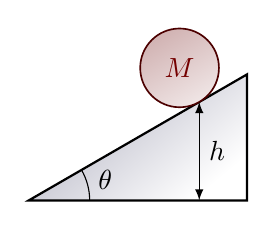
\begin{tikzpicture}
    \def\R{0.5} % disk radius
    \def\W{3.2}  % ground width
    \def\ang{30} % ground angle
    \def\mx{2.5} % mass x position
    \coordinate (X) at (\ang:\mx); % wheel position
    \coordinate (C) at ($(X)+(\ang+90:\R)$); % wheel center
    \draw[thick,top color=blue!20!black!30,bottom color=white,shading angle=\ang+10]
    (0,0) coordinate (O) -- (\ang:\W) coordinate (T) -- ({\W*cos(\ang)},0) coordinate (L) -- cycle;
    \draw[mass] (C) circle(\R) node[myred!70!black] {$M$};
    \draw pic["$\theta$",draw=black,angle radius=22,angle eccentricity=1.3] {angle=L--O--T};
    \draw[<->] (X) --++ (0,{-\mx*sin(\ang)}) node[midway,right] {$h$};
\end{tikzpicture}



\end{document}